\section{Perhitungan}

Fortran90:
diuji dengan menggunakan kompiler berikut: GFortran, g95, ifort, pgi, dan Sun

Potensial eksternal berupa fungsi Gaussian:
\begin{equation}
V_{\mathrm{ext}}(r) = A\exp(-\alpha r^2)
\end{equation}

\begin{figure}[h]
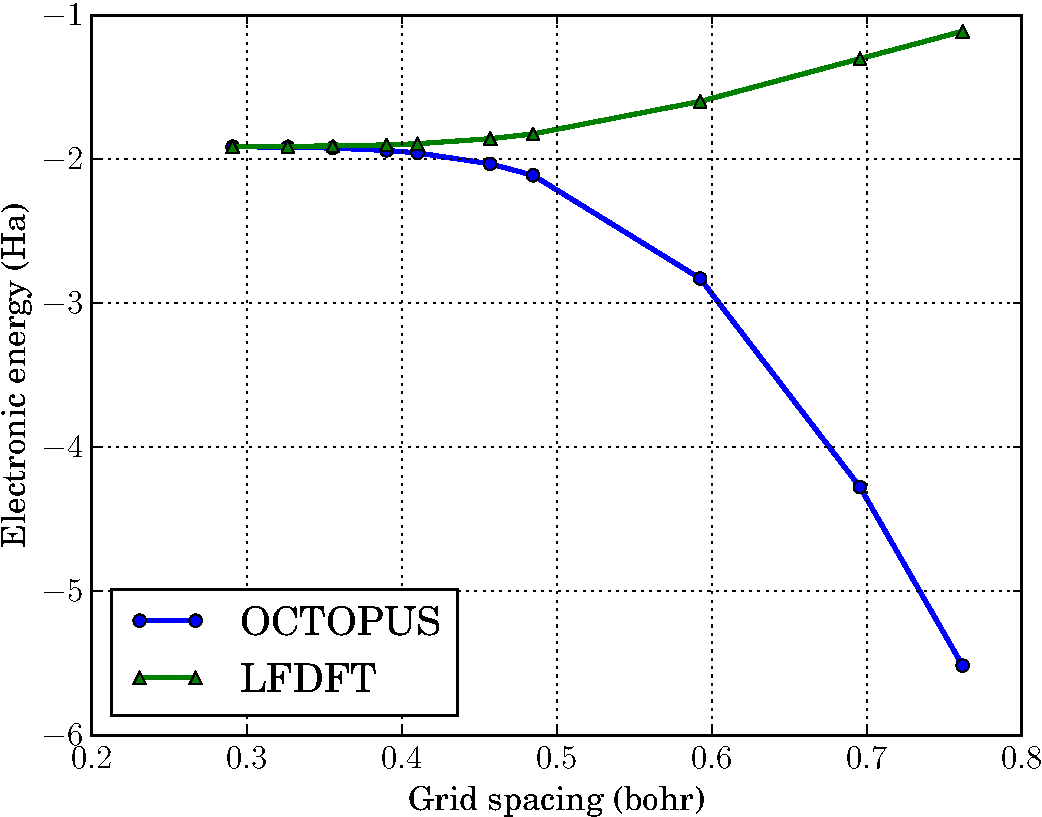
\includegraphics[width=\columnwidth]{images/A_10_alpha_3.pdf}
\end{figure}

Menggunakan bagian lokal dari pseudopotensial HGH
\begin{multline}
V_{\mathrm{ext}}(r) = -\frac{Z_\mathrm{ion}}{r}
\mathrm{erf}\left(\frac{\bar{r}}{\sqrt{2}}\right) +
\exp\left[-\frac{1}{2}\bar{r}^2\right] \\ 
\times
\left[
C_{1} + C_{2}\bar{r}^2 + C_{3}\bar{r}^4 + C_{4}\bar{r}^2
\right]
\end{multline}
dengan $\bar{r} = r/r_{\mathrm{loc}}$

\begin{figure}[h]
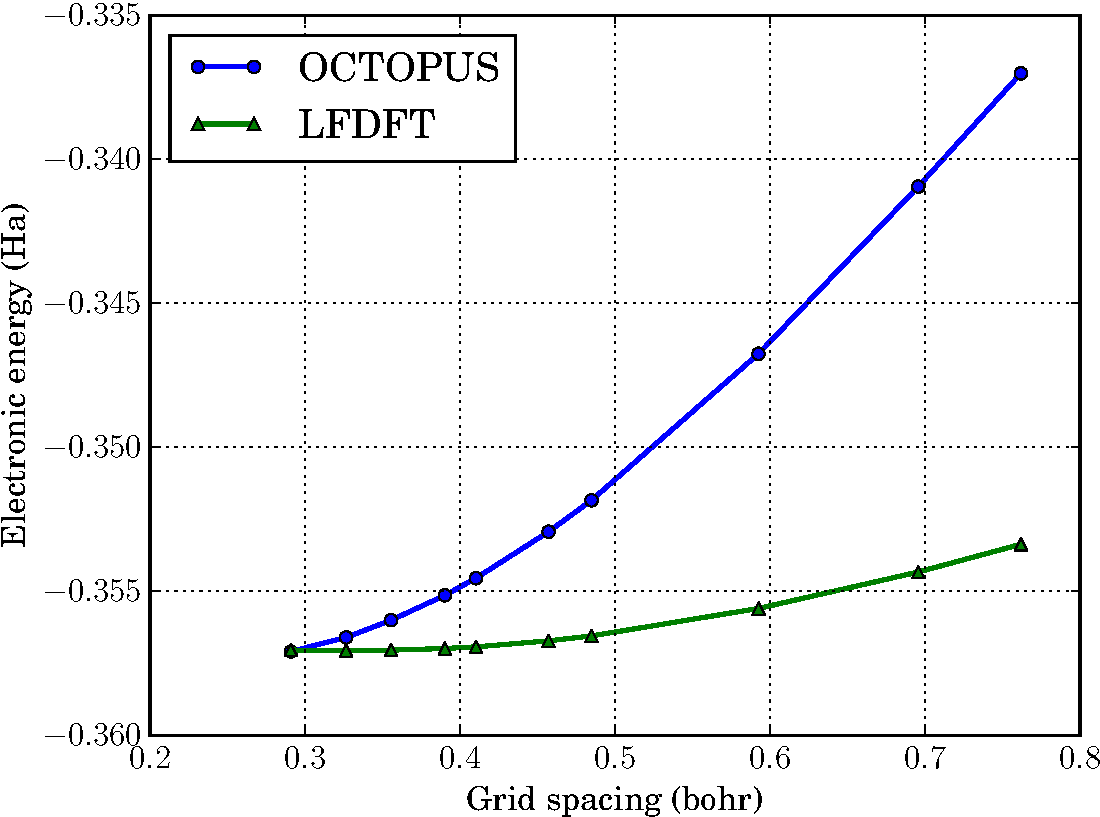
\includegraphics[width=\columnwidth]{images/atom_H.pdf}
\end{figure}

Contoh molekul diatomik: $\ce{H2}$ dan LiH

Visualisasi orbital molekul
